\documentclass{uc3mpracticas}

\usepackage{helvet}
\usepackage{multicol}
\renewcommand{\familydefault}{\sfdefault}
\usepackage{changepage}
\usepackage{geometry}
\usepackage{caption}
\usepackage{xcolor,colortbl}

\definecolor{Gray}{gray}{0.85}
\definecolor{LightCyan}{rgb}{0.88,1,1}
\definecolor{LightGreen}{rgb}{0.29,1,0.39}

\newcolumntype{g}{>{\columncolor{Gray}}l}


%%%%%%%%%%%%%%%%%%%%%%%%%%%%%%%%%%%%%%%%%%%%%%%%%%%%%%%%%%%%%%%%%%%%%%%%%%%%%%%%
%%%                   Plantilla Prácticas UC3M                               %%%
%%%                Universidad Carlos III de Madrid                          %%%
%%%                   Alejandro Valverde Mahou                               %%%
%%%%%%%%%%%%%%%%%%%%%%%%%%%%%%%%%%%%%%%%%%%%%%%%%%%%%%%%%%%%%%%%%%%%%%%%%%%%%%%%

%Permitir cabeceras y pie de páginas personalizados
\pagestyle{fancy}

%Path por defecto de las imágenes
\graphicspath{ {./images/} }

%Declarar formato de encabezado y pie de página de las páginas del documento
\fancypagestyle{doc}{
  %Cabecera
  \headerpr[1]{Problema de Clasificación: Parte II}{}{Redes de Neuronas Artificiales}
  %Pie de Página
  \footerpr{}{\textbf{UC3M}}{{\thepage} de \pageref{LastPage}}
}

%Declarar formato de encabezado y pie del título e indice
\fancypagestyle{titu}{%
  %Cabecera
  \headerpr{}{}{}
  %Pie de Página
  \footerpr{}{}{}
}


\appto\frontmatter{\pagestyle{titu}}
\appto\mainmatter{\pagestyle{doc}}


\begin{document}
  %Comienzo formato título
  \frontmatter


  %Portada 1 (Centrado todo)
  \centeredtitle{Images/LogoUC3M.png}{Grado en Ingeniería Informática}{Curso 2020/2021}{Redes de Neuronas Artificiales}{Problema de Clasificación: Parte II}{Clasificación de imágenes con Redes Convolucionales}

  \vspace{55mm}

  \authors{Alba Reinders Sánchez}{100383444}{Alejandro Valverde Mahou}{100383383}{}{}{}{}

  \newpage

  %Índice
  \tableofcontents

  \newpage

  %Comienzo formato documento general
  \mainmatter

\section{Introducción}

El problema consiste en clasificar imágenes donde las entradas de la red son directamente los píxeles de cada imagen. Se utiliza el conjunto de datos \textit{CIFAR10}, compuesto por \textbf{60000} imágenes en color (3 canales, \textit{RGB}) de \textbf{32x32} píxeles. El conjunto de datos se divide en 50000 imágenes para entrenamiento y 10000 para test.

\vspace{2mm}

Hay un total de \textbf{10 clases} con 6000 imágenes por clase, por lo que en este caso las clases sí están balanceadas, las diferentes clases son:

\begin{itemize}
  \begin{multicols}{5}
  \item 0 $\rightarrow$ \textit{airplane}
  \item 5 $\rightarrow$ \textit{dog}
  \item 1 $\rightarrow$ \textit{automobile}
  \item 6 $\rightarrow$ \textit{frog}
  \item 2 $\rightarrow$ \textit{bird}
  \item 7 $\rightarrow$ \textit{horse}
  \item 3 $\rightarrow$ \textit{cat}
  \item 8 $\rightarrow$ \textit{ship}
  \item 4 $\rightarrow$ \textit{deer}
  \item 9 $\rightarrow$ \textit{truck}
  \end{multicols}
\end{itemize}


El objetivo de la práctica es entrenar diferentes arquitecturas de \textbf{Perceptrón Multicapa} y \textbf{Redes de Neuronas Convolucionales} para analizar cómo influyen sus hiperparámetros en la resolución del problema de clasificación. Además de comparar sus resultados para comprobar cuál de las dos arquitecturas es más efectiva.



\section{Diseño, entrenamiento y evaluación del PM}

Inicialmente se intenta resolver este problema con el método de 'fuerza bruta'. Es decir, se aplana la información de los píxeles de las imágenes de entrada en un único vector y se entrena un \textbf{Perceptrón Multicapa} con estas entradas.

\vspace{2mm}

Para estudiar la eficacia de este acercamiento se realiza una pequeña experimentación probando distintas arquitecturas de red:

\begin{figure}[!h]
\begin{center}
  \begin{tabular}{|c|c|c|c|c|c|}
    \hline
    \rowcolor{Gray}
        \textbf{Arquitectura} & \textbf{\textit{epochs}}& \textbf{\textit{Accuracy} entrenamiento} & \textbf{\textit{Accuracy} test} & \textbf{\textit{Loss} entrenamiento} & \textbf{\textit{Loss} test}\\ \hline \hline
        (50)                  & 25                      &  0.5552                                  &  0.4743                         &  1.2606                              &  1.5040            \\ \hline
        (25)                  & 21                      &  0.5039                                  &  0.4493                         &  1.4128                              &  1.5678            \\ \hline
        (100)                 & 16                      &  0.5543                                  &  0.4922                         &  1.9684                              &  1.4483            \\ \hline
        (100,100)             & 30                      &  0.6442                                  &  0.5045                         &  0.9995                              &  1.4618            \\ \hline
        \rowcolor{LightGreen}
        (100, 100, 100)       & 23                      &  0.5900                                  &  0.5081                         &  1.1478                              &  1.4276            \\ \hline
  \end{tabular}
\end{center}
\caption*{Tabla Experimentos PM}
\end{figure}

En cada uno de los experimentos se ajusta manualmente el número de \textit{epochs} óptimos para encontrar los mejores resultados posibles.

\vspace{2mm}

Se parte de la arquitectura dada en el tutorial y se prueba a modificar sus hiperparámetros a partir de ella. Primero se prueba a disminuir el número de neuronas, lo que no genera mejores resultados. Por tanto se prueba a aumentarlas y el \textit{accuracy} mejora, entonces se decide añadir una capa oculta más y también genera mejores resultados.

\vspace{1mm}

Como último experimento se configura una red con 3 capas ocultas de 100 neuronas cada una, este obtiene los mejores resultados. Sin embargo, el \textit{accuracy} en test que alcanza se queda estancado entorno a 0,5.

\vspace{2mm}

Tras esta experimentación se puede concluir que aumentar la complejidad de la arquitectura de la red, tanto en capas ocultas como en neuronas, hace que genere mejores resultados. Aunque no consigue superar un umbral, por lo que la utilización del \textit{PM} para resolver este problema no es del todo eficaz.



\begin{figure}[!h]
\centering
\begin{minipage}{.52\textwidth}
  \centering
  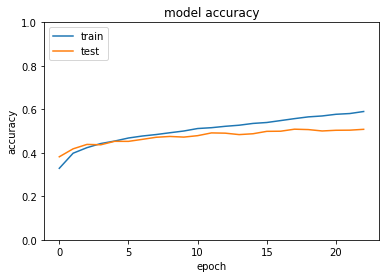
\includegraphics[width=.8\linewidth]{Images/accuracyPM.png}
  \caption*{\textit{Accuracy} en entrenamiento y test del \textit{PM}}
\end{minipage}%
\begin{minipage}{.52\textwidth}
  \centering
  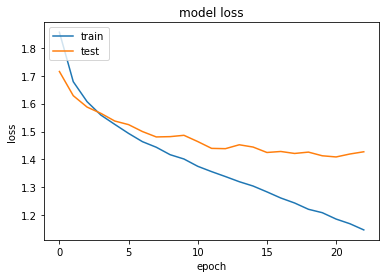
\includegraphics[width=.8\linewidth]{Images/lossPM.png}
  \caption*{\textit{Loss} en entrenamiento y test del \textit{PM}}
\end{minipage}
\end{figure}


\begin{figure}[!h]
\begin{center}
  \begin{tabular}{|g|c|c|c|c|c|c|c|c|c|c|}
    \hline
    \rowcolor{Gray}
    Real $\;$\textbackslash  $\;$ Predicho  & \textbf{Airplane} & \textbf{Automobile} & \textbf{Bird} & \textbf{Cat} & \textbf{Deer} & \textbf{Dog} & \textbf{Frog} & \textbf{Horse} & \textbf{Ship} & \textbf{Truck} \\ \hline
            \textbf{Airplane}               &                 &                   &             &            &             &            &             &              &             &                \\ \hline
            \textbf{Automobile}             &                 &                   &             &            &             &            &             &              &             &                \\ \hline
            \textbf{Bird}                   &                 &                   &             &            &             &            &             &              &             &                \\ \hline
            \textbf{Cat}                    &                 &                   &             &            &             &            &             &              &             &                \\ \hline
            \textbf{Deer}                   &                 &                   &             &            &             &            &             &              &             &                \\ \hline
            \textbf{Dog}                    &                 &                   &             &            &             &            &             &              &             &                \\ \hline
            \textbf{Frog}                   &                 &                   &             &            &             &            &             &              &             &                \\ \hline
            \textbf{Horse}                  &                 &                   &             &            &             &            &             &              &             &                \\ \hline
            \textbf{Ship}                   &                 &                   &             &            &             &            &             &              &             &                \\ \hline
            \textbf{Truck}                  &                 &                   &             &            &             &            &             &              &             &                \\ \hline
      \end{tabular}
\end{center}
\caption*{Matriz de confusión mejor experimeto \textit{PM}}
\end{figure}



\section{Diseño, entrenamiento y evaluación de la CNN}

\begin{figure}[!h]
\begin{center}
  \begin{tabular}{|g|c|c|c|c|c|c|c|c|c|c|}
    \hline
    \rowcolor{Gray}
    Real $\;$\textbackslash  $\;$ Predicho  & \textbf{Airplane} & \textbf{Automobile} & \textbf{Bird} & \textbf{Cat} & \textbf{Deer} & \textbf{Dog} & \textbf{Frog} & \textbf{Horse} & \textbf{Ship} & \textbf{Truck} \\ \hline
            \textbf{Airplane}               &                 &                   &             &            &             &            &             &              &             &                \\ \hline
            \textbf{Automobile}             &                 &                   &             &            &             &            &             &              &             &                \\ \hline
            \textbf{Bird}                   &                 &                   &             &            &             &            &             &              &             &                \\ \hline
            \textbf{Cat}                    &                 &                   &             &            &             &            &             &              &             &                \\ \hline
            \textbf{Deer}                   &                 &                   &             &            &             &            &             &              &             &                \\ \hline
            \textbf{Dog}                    &                 &                   &             &            &             &            &             &              &             &                \\ \hline
            \textbf{Frog}                   &                 &                   &             &            &             &            &             &              &             &                \\ \hline
            \textbf{Horse}                  &                 &                   &             &            &             &            &             &              &             &                \\ \hline
            \textbf{Ship}                   &                 &                   &             &            &             &            &             &              &             &                \\ \hline
            \textbf{Truck}                  &                 &                   &             &            &             &            &             &              &             &                \\ \hline
      \end{tabular}
\end{center}
\caption*{Matriz de confusión mejor experimeto \textit{CNN}}
\end{figure}

\section{Comparación PM y CNN}




\section{Conclusión}









\end{document}
